\documentclass[journal,12pt,onecolumn]{IEEEtran}
\usepackage{graphicx, float}
\graphicspath{{Figs/}}
\usepackage{multicol}
\usepackage{parskip}
\usepackage{titlesec}
\usepackage{color}
\usepackage{enumitem}
\usepackage{amsmath,amssymb,amsfonts,amsthm}
\usepackage{array}
\usepackage{booktabs}
\usepackage[table]{xcolor}
\usepackage{longtable}
\usepackage{gensymb}
\usepackage{cite}
\usepackage{algorithmic}
\usepackage{textcomp}
\usepackage{txfonts}
\usepackage{listings}
\usepackage{mathtools}
\usepackage{comment}
\usepackage{tkz-euclide}
\usepackage[breaklinks=true]{hyperref}
\usepackage{gvv}
\usepackage[latin1]{inputenc}
\usetikzlibrary{arrows.meta, positioning}
\usepackage{xparse}
\usepackage{calc}
\usepackage{multirow}
\usepackage{hhline}
\usepackage{ifthen}
\usepackage{lscape}
\usepackage{tabularx}
\usepackage{circuitikz}
\usepackage{tikz}
\newtheorem{problem}{Problem}
\newtheorem{theorem}{Theorem}[section]
\newtheorem{proposition}{Proposition}[section]
\newtheorem{lemma}{Lemma}[section]
\newtheorem{corollary}[theorem]{Corollary}
\newtheorem{example}{Example}[section]
\newtheorem{definition}[problem]{Definition}
\newcommand{\BEQA}{\begin{eqnarray}}
\newcommand{\EEQA}{\end{eqnarray}}
\theoremstyle{remark}
\usepackage{pgfplots}
\pgfplotsset{compat=1.18}

\usepackage{tikz}

\title{GATE EE 2018}
\author{ai25btech11028 R.Manohar}
\begin{document}
\maketitle
\subsection{Q.1-Q.5 carry one mark each}
\begin{enumerate}
 \item "Since you have gone off the \_\_\_\_\_\_\_\_, the \_\_\_\_\_\_\_\_ sand is likely to damage the car." 
    The words that best fill the blanks in the above sentence are
    \begin{multicols}{4}
    \begin{enumerate}
        \item coarse, coarse
        \item bourse, coarse
        \item course, coarse
        \item coarse, course
    \end{enumerate}
    \end{multicols}
    \hfill{(GATE EE 2018)}

    \item "A common misconception among writers is that sentence structure mirrors thought; the more \_\_\_\_\_\_\_\_\_ the structure, the more complicated the ideas."
    The word that best fills the blank in the above sentence is
    \begin{multicols}{4}
    \begin{enumerate}
        \item detailed
        \item simple
        \item clear
        \item convoluted
    \end{enumerate}
   \end{multicols}
    \hfill{(GATE EE 2018)}

    \item The three roots of the equation $f(x) = 0$ are $x = \{-2, 0, 3\}$. What are the three values of $x$ for which $f(x - 3) = 0$?
    \begin{enumerate}
    \begin{multicols}{4}
        \item $-5, -3, 0$
        \item $-2, 0, 3$
        \item $0, 6, 8$
        \item $1, 3, 6$
        \end{multicols}
    \end{enumerate}
     \hfill{(GATE EE 2018)}

    \item For what values of $k$ given below is $\frac{(k+2)^{2}}{k-3}$ an integer?
    \begin{multicols}{4}
    \begin{enumerate}
        \item 4, 8, 18
        \item 4, 10, 16
        \item 4, 8, 28
        \item 8, 26, 28
    \end{enumerate}
    \end{multicols}
     \hfill{(GATE EE 2018)}
    
    \item Functions $F(a, b)$ and $G(a, b)$ are defined as follows:
    \begin{align*}
    F(a, b) = (a - b)^{2}
    \end{align*}
    and 
    \begin{align*}
    G(a, b) = |a - b|
    \end{align*}
    , where $|x|$ represents the absolute value of $x$. \\
    What would be the value of $G(F(1, 3), G(1, 3))$?
    \begin{multicols}{4}
    \begin{enumerate}
        \item 2
        \item 4
        \item 6
        \item 36
    \end{enumerate}
    \end{multicols}
    \hfill{(GATE EE 2018)}

\subsection{Q.6-Q.10 carry one mark each}

\item An e-mail password must contain three characters. The password has to contain one numeral from 0 to 9, one upper case and one lower case character from the English alphabet. How many distinct passwords are possible?
\begin{multicols}{4}
    \begin{enumerate}
        \item 6,760
        \item 13,520
        \item 40,560
        \item 1,05,456
    \end{enumerate}
    \end{multicols}

    \hfill{(GATE EE 2018)}
    \item In a certain code, AMCF is written as EQQJ and NKUF is written as ROYJ. How will DHLP be written in that code?
    \begin{multicols}{4}
    \begin{enumerate}
        \item RSTN
        \item TLPH
        \item HLPT
        \item XSVR
    \end{enumerate}
    \end{multicols}
     \hfill{(GATE EE 2018)}
    
    \item A class of twelve children has two more boys than girls. A group of three children are randomly picked from this class to accompany the teacher on a field trip. What is the probability that the group accompanying the teacher contains more girls than boys?
    \begin{multicols}{4}
    \begin{enumerate}
        \item 0
        \item $\frac{5}{864}$
        \item $\frac{5}{864}$
        \item $\frac{5}{12}$
    \end{enumerate}
    \end{multicols}
     \hfill{(GATE EE 2018)}
    
    \item A designer uses marbles of four different colours for his designs. The cost of each marble is the same, irrespective of the colour. The table below shows the percentages of marbles of each colour used in the current design. The cost of each marble increased by 25\%. Therefore, the designer decided to reduce equal numbers of marbles of each colour to keep the total cost unchanged. What is the percentage of blue marbles in the new design?
    \begin{center}
        \begin{tabular}{|l|c|c|c|c|}
            \hline
            \textbf{Blue} & \textbf{Black} & \textbf{Red} & \textbf{Yellow} \\
            \textbf{40\%} & \textbf{25\%} & \textbf{20\%} & \textbf{15\%} \\
            \hline
        \end{tabular}
    \end{center}
    \begin{multicols}{4}
    \begin{enumerate}
        \item 35.75
        \item 40.25
        \item 43.75
        \item 46.25
    \end{enumerate}
    \end{multicols}
    \hfill{(GATE EE 2018)}
    
    \item P, Q, R and S crossed a lake in a boat that can hold a maximum of two persons, with only one set of oars. The following additional facts are available:
    \begin{enumerate}
        \item The boat held two persons on each of the three forward trips across the lake and one person on each of the two return trips.
        \item P is unable to row when someone else is in the boat.
        \item Q is unable to row with anyone else except R.
        \item Each person rowed for at least one trip.
        \item Only one person can row during a trip.
    \end{enumerate}
    Who rowed twice?
    \begin{enumerate}
        \item P
        \item Q
        \item R
        \item S
    \end{enumerate}
\end{enumerate}
\hfill{(GATE EE 2018)}

\vspace{1cm}
\begin{center}
    END OF QUESTION PAPER
\end{center}


\begin{enumerate}
\subsection{Q.1-Q.25 carry one mark each}
\item A single-phase 100 kVA, 1000 V / 100 V, 50 Hz transformer has a voltage drop of 5\% across its series impedance at full load. Of this, 3\% is due to resistance. The percentage regulation of the transformer at full load with 0.8 lagging power factor is
\begin{multicols}{4}
    \begin{enumerate}
        \item 4.8
        \item 6.8
        \item 8.8
        \item 10.8
    \end{enumerate}
    \end{multicols}
\hfill{(GATE EE 2018)}

    \item In a salient pole synchronous motor, the developed reluctance torque attains the maximum value when the load angle in electrical degrees is
    \begin{multicols}{4}
    \begin{enumerate}
        \item 0
        \item 45
        \item 60
        \item 90
    \end{enumerate}
    \end{multicols}
\hfill{(GATE EE 2018)}
    \item A single phase fully controlled rectifier is supplying a load with an anti-parallel diode as shown in the figure. All switches and diodes are ideal. Which one of the following is true for instantaneous load voltage and current?
  \begin{figure}[H]
    \centering
    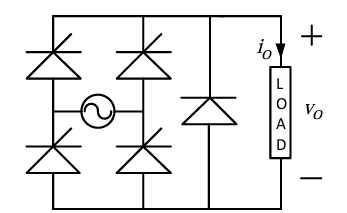
\includegraphics[]{figs/Q.3.png}
    \caption{}
    \label{fig:1}
\end{figure}
    \begin{enumerate}
        \item $v_{O} \geq 0 \text{ \& } i_{O} < 0$
        \item $v_{O} < 0 \text{ \& } i_{O} < 0$
        \item $v_{O} \geq 0 \text{ \& } i_{O} \geq 0$
        \item $v_{O} < 0 \text{ \& } i_{O} \geq 0$
    \end{enumerate}
\hfill{(GATE EE 2018)}
    \item Four power semiconductor devices are shown in the figure along with their relevant terminals. The device(s) that can carry dc current continuously in the direction shown when gated appropriately is (are)
    \begin{figure}[H]
    \centering
    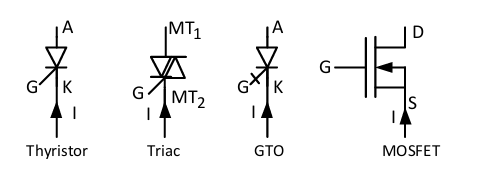
\includegraphics[]{figs/Q.4.png}
    \caption{}
    \label{fig:2}
\end{figure}
\begin{multicols}{2}
    \begin{enumerate}
        \item Triac only
        \item Triac and MOSFET
        \item Triac and GTO
        \item Thyristor and Triac
    \end{enumerate}
    \end{multicols}
\hfill{(GATE EE 2018)}

    \item Two wattmeter method is used for measurement of power in a balanced three-phase load supplied from a balanced three-phase system. If one of the wattmeters reads half of the other (both positive), then the power factor of the load is
    \begin{multicols}{4}
    \begin{enumerate}
        \item 0.532
        \item 0.632
        \item 0.707
        \item 0.866
    \end{enumerate}
    \end{multicols}
\hfill{(GATE EE 2018)}

    \item Consider a lossy transmission line with $V_{S}$ and $V_{R}$ as the sending and receiving end voltages, respectively. $Z$ and $X$ are the series impedance and reactance of the line, respectively. The steady-state stability limit for the transmission line will be
    \begin{enumerate}
        \item greater than $\frac{|V_{S}| |V_{R}|}{|X|}$
        \item less than $\frac{|V_{S}| |V_{R}|}{|X|}$
        \item equal to $\frac{|V_{S}| |V_{R}|}{|X|}$
        \item equal to $\frac{|V_{S}| |V_{R}|}{|Z|}$
    \end{enumerate}
\hfill{(GATE EE 2018)}

    \item The graph of a network has 8 nodes and 5 independent loops. The number of branches of the graph is
    \begin{multicols}{4}
    \begin{enumerate}
        \item 11
        \item 12
        \item 13
        \item 14
    \end{enumerate}
    \end{multicols}
\hfill{(GATE EE 2018)}

    \item In the figure, the voltages are $v_{1}(t) = 100 \cos(\omega t)$, $v_{2}(t) = 100 \cos(\omega t + \pi/18)$ and $v_{3}(t) = 100 \cos(\omega t + \pi/36)$. The circuit is in sinusoidal steady state, and $R > 0$. $P_{1}, P_{2}$ and $P_{3}$ are the average power outputs. Which one of the following statements is true?
    \begin{figure}[H]
    \centering
    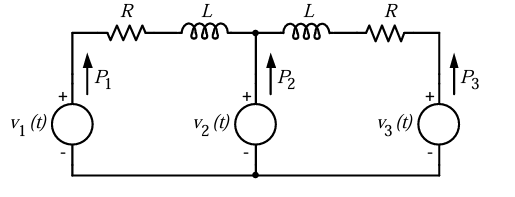
\includegraphics[]{figs/Q.8.png}
    \caption{}
    \label{fig:3}
\end{figure}
    \begin{multicols}{2}
    \begin{enumerate}
        \item $P_{1} = P_{2} = P_{3} = 0$
        \item $P_{1} < 0, P_{2} > 0, P_{3} > 0$
        \item $P_{1} < 0, P_{2} > 0, P_{3} < 0$
        \item $P_{1} > 0, P_{2} < 0, P_{3} > 0$
    \end{enumerate}
    \end{multicols}
\hfill{(GATE EE 2018)}

    \item Match the transfer functions of the second-order systems with the nature of the systems given below:
    \begin{tabular}{|l|l|}
        \hline
        \textbf{Transfer functions} & \textbf{Nature of system} \\
        \hline
        P: $\frac{15}{s^{2}+2s+15}$ & I: Overdamped \\
        Q: $\frac{25}{s^{2}+10s+25}$ & II: Critically damped \\
        R: $\frac{35}{s^{2}+18s+35}$ & III: Underdamped \\
        \hline
    \end{tabular}
    \begin{multicols}{2}
    \begin{enumerate}
        \item P-I, Q-II, R-III
        \item P-II, Q-I, R-III
        \item P-III, Q-II, R-I
        \item P-III, Q-I, R-II
    \end{enumerate}
    \end{multicols}
\hfill{(GATE EE 2018)}

    \item A positive charge of 1 nC is placed at (0, 0, 0.2) where all dimensions are in metres. Consider the $x$-$y$ plane to be a conducting ground plane. The magnitude of the $z$ component of the E field at (0, 0, 0.1) is closest t
    \begin{multicols}{4}
    \begin{enumerate}
        \item 899.18 V/m
        \item -899.18 V/m
        \item 99.09 V/m
        \item -999.09 V/m
    \end{enumerate}
\end{multicols}  
\hfill{(GATE EE 2018)}

    \item Let $f$ be a real-valued function of a real variable defined as 
    \begin{align*}
    f(x) = x - \lfloor x \rfloor 
    \end{align*}
    where $\lfloor x \rfloor$ denotes the largest integer less than or equal to $x$. Which one of the following statements is true?
    \begin{enumerate}
        \item $f(x)$ is discontinuous at $x=0$.
        \item $f(x)$ is continuous but not differentiable at $x=0$.
        \item $f(x)$ is differentiable but its first derivative is not continuous at $x=0$.
        \item $f(x)$ is differentiable but its first derivative is not differentiable at $x=0$.
    \end{enumerate}
    \hfill{(GATE EE 2018)}

    \item The value of the directional derivative of the function 
    \begin{align*}
    \phi(x, y, z) = xy^{2} + yz^{2} + zx^{2}
    \end{align*}
    at the point $(2, -1, 1)$ in the direction of the vector $\vec{p} = \vec{i} + 2\vec{j} + 2\vec{k}$ is
    \begin{multicols}{4}
    \begin{enumerate}
        \item 1
        \item 0.95
        \item 0.93
        \item 0.9
    \end{enumerate}
    \end{multicols}
    \hfill{(GATE EE 2018)}

    \item The value of the integral $\oint_{C} \frac{e^{z}}{z+4} dz$ in counter clockwise direction around a circle $C$ of radius 4 with center at the point $z = -2$ is
    \begin{multicols}{4}
    \begin{enumerate}
        \item $\frac{\pi i}{2}$
        \item $2\pi i$
        \item $\frac{\pi i}{2}$
        \item $-2\pi i$
    \end{enumerate}
    \end{multicols}
    \hfill{(GATE EE 2018)}

    \item In the logic circuit shown in the figure, $Y$ is given by
    \begin{figure}[H]
    \centering
    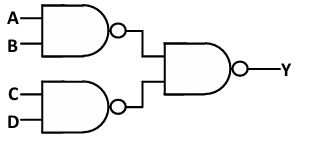
\includegraphics[]{figs/Q.14.png}
    \caption{}
    \label{fig:4}
\end{figure}
    \begin{multicols}{2}
    \begin{enumerate}
        \item $Y = \bar{A} B C D$
        \item $Y = (\bar{A} + B)(C + D)$
        \item $Y = \bar{A} + B + C + D$
        \item $Y = AB + CD$
    \end{enumerate}
    \end{multicols}
    \hfill{(GATE EE 2018)}

    \item The op-amp shown in the figure is ideal. The input impedance $Z_{in}$ is given by
    \begin{figure}[H]
    \centering
    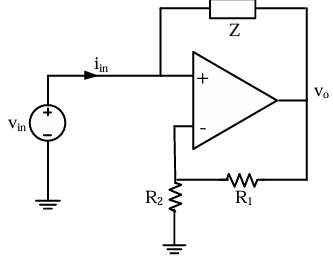
\includegraphics[]{figs/Q.15.png}
    \caption{}
    \label{fig:5}
\end{figure}
    \begin{multicols}{2}
    \begin{enumerate}
        \item $Z \frac{R_{1}}{R_{2}}$
        \item $-Z \frac{R_{2}}{R_{1}}$
        \item $Z$
        \item $-Z \frac{R_{1}}{R_{1}+R_{2}}$
    \end{enumerate}
    \end{multicols}
    \hfill{(GATE EE 2018)}

    \item A continuous-time input signal $x(t)$ is an eigenfunction of an LTI system, if the output is
    \begin{enumerate}
        \item $k \phi(t)$ where $k$ is an eigenvalue
        \item $\phi(t) e^{\omega t}$ where $\omega$ is an eigenvalue and $e^{\omega t}$ is a complex exponential signal
        \item $x(t) e^{\omega t}$ where $e^{\omega t}$ is a complex exponential signal
        \item $H(\omega) \phi(t)$ where $H(\omega)$ is a frequency response of the system
    \end{enumerate}
    \hfill{(GATE EE 2018)}

    \item Consider a non-singular $2 \times 2$ square matrix $A$. If $\text{trace}(A) = 4$ and $\text{trace}(A^{2}) = 5$, the determinant of the matrix $A$ is \_\_\_\_\_\_\_\_\_\_ (up to 1 decimal place).
    \hfill{(GATE EE 2018)}
    
    \item Let $f$ be a real-valued function of a real variable defined as $f(x) = \lfloor x \rfloor - x$, where $\lfloor x \rfloor$ denotes the greatest integer less than or equal to $x$. The value of $\int_{-1.25}^{1.25} f(x) dx$ is \_\_\_\_\_\_\_\_\_\_\_\_\_\_ (up to 2 decimal places).
    \hfill{(GATE EE 2018)}

    \item In the two-port network shown, the $h_{11}$ parameter where $h_{11} = \frac{V_{1}}{I_{1}}$, when $V_{2}=0$ in ohms is \_\_\_\_\_\_\_\_\_\_\_\_\_\_ (up to 2 decimal places).
   \begin{figure}[H]
    \centering
    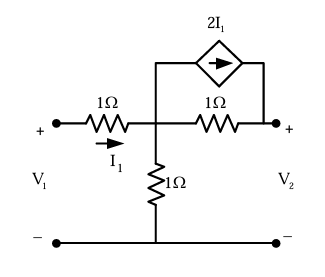
\includegraphics[]{figs/Q.19.png}
    \caption{}
    \label{fig:6}
\end{figure}
\hfill{(GATE EE 2018)}

    \item The series impedance matrix of a short three-phase transmission line in phase coordinates is \myvec{ 
    Z_{ss} & Z_{sm} & Z_{sm} \\ 
    Z_{sm} & Z_{ss} & Z_{sm} \\ 
    Z_{sm} & Z_{sm} & Z_{ss} 
}
. If the positive sequence impedance is $(1 + j10) \Omega$, and the zero sequence is $(4 + j31) \Omega$, then the imaginary part of $Z_{se}$ (in $\Omega$) is \_\_\_\_\_\_\_\_\_\_\_\_\_\_ (up to 2 decimal places).
   \hfill{(GATE EE 2018)} 

    \item The positive, negative and zero sequence impedances of a 125 MVA, three-phase, 15.5 kV, star-grounded, 60 Hz generator are $j0.1$ pu, $j0.05$ pu and $j0.01$ pu respectively on the machine rating base. The machine is unloaded and working at the rated terminal voltage. If the grounding impedance of the generator is $j0.01$ pu, then the magnitude of fault current for a b-phase to ground fault (in kA) is \_\_\_\_\_\_\_\_\_\_\_\_\_\_ (up to 2 decimal places).
  \hfill{(GATE EE 2018)}  
    
    \item A 1000 $\times$ 1000 bus admittance matrix for an electric power system has 8000 non-zero elements. The minimum number of branches (transmission lines and transformers) in this system are \_\_\_\_\_\_\_\_\_\_\_\_\_\_ (up to 2 decimal places).
   \hfill{(GATE EE 2018)} 

    \item The waveform of the current drawn by a semi-converter from a sinusoidal AC voltage source is shown in the figure. If $I_s = 20$ A, the rms value of fundamental component of the current is \_\_\_\_\_\_\_\_\_\_\_\_\_\_ A (up to 2 decimal places).
    \begin{figure}[H]
    \centering
    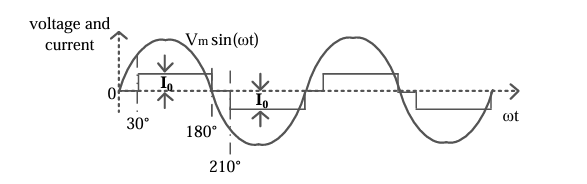
\includegraphics[]{figs/Q.23.png}
    \caption{}
    \label{fig:7}
\end{figure}
   \hfill{(GATE EE 2018)} 
    
    \item A separately excited dc motor has an armature resistance $R_{a} = 0.05 \Omega$. The field excitation is kept constant. At an armature voltage of 100 V, the motor produces a torque of 500 Nm at zero speed. Neglecting all mechanical losses, the no-load speed of the motor (in rad/s) for an armature voltage of 150 V is \_\_\_\_\_\_\_\_\_\_\_\_\_\_ (up to 2 decimal places).
   \hfill{(GATE EE 2018)} 
    
    \item Consider a unity feedback system with forward transfer function given by
    \begin{align*}
     G(s) = \frac{1}{(s+1)(s+2)} 
    \end{align*}
    The steady-state error in the output of the system for a unit-step input is \_\_\_\_\_\_\_\_\_\_\_\_\_\_ (up to 2 decimal places).
\hfill{(GATE EE 2018)}

\subsection{Q.26-Q.55 carry two marks each}
\item A transformer with toroidal core of permeability $\mu$ is shown in the figure. Assuming uniform flux density across the circular core cross-section of radius $r \ll R$, and neglecting any leakage flux, the best estimate for the mean radius $R$ is
\begin{figure}[H]
    \centering
    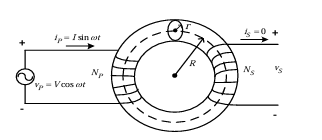
\includegraphics[]{figs/Q.26.png}
    \caption{}
    \label{fig:8}
\end{figure}
\begin{multicols}{4}
\begin{enumerate}
    \item $\dfrac{\mu V r^2 N_p^2 \omega}{I}$
    \item $\dfrac{\mu I r^2 N_p N_s \omega}{V}$
    \item $\dfrac{\mu V r^2 N_p \omega}{2I}$
    \item $\dfrac{\mu I r^2 N_p^2}{2V}$
\end{enumerate}
\end{multicols}
\hfill{(GATE EE 2018)}

\item A 0-1 Ampere moving iron ammeter has an internal resistance of 50 m$\Omega$ and inductance of 0.1 mH. A shunt coil is connected to extend its range to 0-10 Ampere for all operating frequencies. The time constant in milliseconds and resistance in m$\Omega$ of the shunt coil respectively are
\begin{multicols}{4}
\begin{enumerate}
    \item 2, 5.55
    \item 2, 1
    \item 2.18, 0.55
    \item 11.1, 2
\end{enumerate}
\end{multicols}
\hfill{(GATE EE 2018)}

\item The positive, negative and zero sequence impedances of a three phase generator are $Z_1, Z_2$ and $Z_0$ respectively. For a line-to-line fault with fault impedance $Z_f$, the fault current is $I_{f1} = k I_f$, where $I_f$ is the fault current with zero fault impedance. The relation between $Z_f$ and $k$ is
\begin{multicols}{4}
\begin{enumerate}
    \item $Z_f = \dfrac{(Z_1+Z_2)(1-k)}{k}$
    \item $Z_f = \dfrac{(Z_1+Z_2)(1+k)}{k}$
    \item $Z_f = \dfrac{(Z_1+Z_2)k}{1-k}$
    \item $Z_f = \dfrac{(Z_1+Z_2)k}{1+k}$
\end{enumerate}
\end{multicols}
\hfill{(GATE EE 2018)}

\item Consider the two bus power system network with given loads as shown in the figure. All the values shown in the figure are in per unit. The reactive power supplied by generator $G_1$ and $G_2$ are $Q_{G1}$ and $Q_{G2}$ respectively. The per unit values of $Q_{G1}$, $Q_{G2}$, and line reactive power loss ($Q_{loss}$) respectively are
\begin{figure}[H]
    \centering
    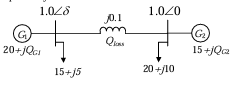
\includegraphics[]{figs/Q.29.png}
    \caption{}
    \label{fig:9}
\end{figure}
\begin{multicols}{2}
\begin{enumerate}
    \item 5.00, 12.68, 2.68
    \item 6.34, 10.00, 1.34
    \item 6.34, 11.34, 2.68
    \item 5.00, 11.34, 1.34
\end{enumerate}
\end{multicols}
\hfill{(GATE EE 2018)}

\item The per-unit power output of a salient-pole generator which is connected to an infinite bus, is given by the expression, $P = 1.4 \sin \delta + 0.15 \sin 2\delta$, where $\delta$ is the load angle. Newton-Raphson method is used to calculate the value of $\delta$ for $P = 0.8$ pu. If the initial guess is $30^\circ$, then its value (in degree) at the end of the first iteration is
\begin{multicols}{4}
\begin{enumerate}
    \item $15^\circ$
    \item $28.48^\circ$
    \item $28.74^\circ$
    \item $31.20^\circ$
\end{enumerate}
\end{multicols}
\hfill{(GATE EE 2018)}

\item A DC voltage source is connected to a series L-C circuit by turning on the switch S at time $t=0$ as shown in the figure. Assume $i(0)=0, v(0)=0$. Which one of the following circular loci represents the plot of $i(t)$ versus $v(t)$?
\begin{figure}[H]
    \centering
    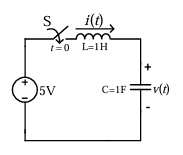
\includegraphics[]{figs/Q.31.png}
    \caption{}
    \label{fig:10}
\end{figure}
\begin{multicols}{4}
\begin{enumerate}
    \item 
    \begin{figure}[H]
    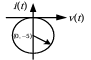
\includegraphics[]{figs/Q.31-OPTION-1.png}
    \label{fig:11}
    \end{figure}
   
    \item 
    \begin{figure}[H]
    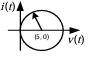
\includegraphics[]{figs/Q.31-OPTION-2.png}
    \label{fig:12}
    \end{figure}
   
    \item 
    \begin{figure}[H]
    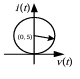
\includegraphics[]{figs/Q.31-OPTION-3.png}
    \label{fig:13}
    \end{figure}
    
    \item 
    \begin{figure}[H]
    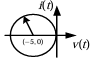
\includegraphics[]{figs/Q.31-OPTION-4.png}
    \label{fig:14}
    \end{figure}
\end{enumerate}
\end{multicols}
\hfill{(GATE EE 2018)}

\item The equivalent impedance $Z_{eq}$ for the infinite ladder circuit shown in the figure is
\begin{figure}[H]
    \centering
    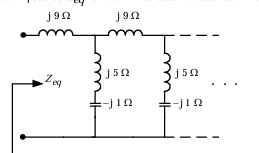
\includegraphics[]{figs/Q.32.png}
    \caption{}
    \label{fig:15}
\end{figure}
\begin{multicols}{4}
\begin{enumerate}
    \item $j12 \, \Omega$
    \item $-j12 \, \Omega$
    \item $j13 \, \Omega$
    \item $13 \, \Omega$
\end{enumerate}
\end{multicols}
\hfill{(GATE EE 2018)}

\item Consider a system governed by the following equations
\begin{align*}
\frac{dx_1(t)}{dt} &= x_2(t) - x_1(t) \\
\frac{dx_2(t)}{dt} &= x_1(t) - x_2(t)
\end{align*}
The initial conditions are such that $x_1(0) < x_2(0) < \infty$. Let $x_{1f} = \lim_{t \to \infty} x_1(t)$ and $x_{2f} = \lim_{t \to \infty} x_2(t)$. Which one of the following is true?
\begin{multicols}{4}
\begin{enumerate}
    \item $x_{1f} < x_{2f} < \infty$
    \item $x_{2f} < x_{1f} < \infty$
    \item $x_{1f} = x_{2f} < \infty$
    \item $x_{1f} = x_{2f} = \infty$
\end{enumerate}
\end{multicols}
\hfill{(GATE EE 2018)}

\item The number of roots of the polynomial, $s^7 + s^6 + 7s^5 + 14s^4 + 31s^3 + 73s^2 + 25s + 200$, in the open left half of the complex plane is
\begin{multicols}{4}
\begin{enumerate}
    \item 3
    \item 4
    \item 5
    \item 6
\end{enumerate}
\end{multicols}
\hfill{(GATE EE 2018)}

\item If C is a circle $|z|=4$ and $f(z) = \dfrac{z^2}{(z^2-3z+2)^2}$, then $\oint_C f(z) dz$ is
\begin{multicols}{4}
\begin{enumerate}
    \item 1
    \item 0
    \item -1
    \item -2
\end{enumerate}
\end{multicols}
\hfill{(GATE EE 2018)}

\item Which one of the following statements is true about the digital circuit shown in the figure
\begin{figure}[H]
    \centering
    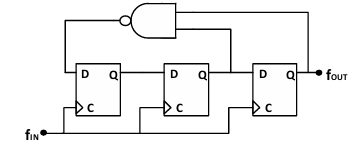
\includegraphics[]{figs/Q.36.png}
    \caption{}
    \label{fig:16}
\end{figure}
\begin{enumerate}
    \item It can be used for dividing the input frequency by 3.
    \item It can be used for dividing the input frequency by 5.
    \item It can be used for dividing the input frequency by 7.
    \item It cannot be reliably used as a frequency divider due to disjoint internal cycles.
\end{enumerate}
\hfill{(GATE EE 2018)}

\item Digital input signals A, B, C with A as the MSB and C as the LSB are used to realize the Boolean function $F = m_0 + m_2 + m_3 + m_5 + m_7$, where $m_i$ denotes the $i^{th}$ minterm. In addition, F has a don't care for $m_1$. The simplified expression for F is given by
\begin{multicols}{2}
\begin{enumerate}
    \item $\bar{A}\bar{C} + \bar{B}C + AC$
    \item $\bar{A} + C$
    \item $\bar{C} + A$
    \item $\bar{A}C + BC + A\bar{C}$
\end{enumerate}
\end{multicols}
\hfill{(GATE EE 2018)}

\item Consider the two continuous-time signals defined below:
\begin{align*}
x_1(t) &= \begin{cases} |t|, & -1 \le t \le 1 \\ 0, & \text{otherwise} \end{cases}, \quad
x_2(t) = \begin{cases} 1-|t|, & -1 \le t \le 1 \\ 0, & \text{otherwise} \end{cases}
\end{align*}
These signals are sampled with a sampling period of $T = 0.25$ seconds to obtain discrete-time signals $x_1[n]$ and $x_2[n]$, respectively. Which one of the following statements is true?
\begin{enumerate}
    \item The energy of $x_1[n]$ is greater than the energy of $x_2[n]$.
    \item The energy of $x_2[n]$ is greater than the energy of $x_1[n]$.
    \item $x_1[n]$ and $x_2[n]$ have equal energies.
    \item Neither $x_1[n]$ nor $x_2[n]$ is a finite-energy signal.
\end{enumerate}
\hfill{(GATE EE 2018)}

\item The signal energy of the continuous-time signal $x(t) = [u(t-1)u(t-1)] - [u(t-2)u(t-2)] - [u(t-3)u(t-3)] + [u(t-4)u(t-4)]$ is
\begin{multicols}{4}
\begin{enumerate}
    \item 11/3
    \item 7/3
    \item 1/3
    \item 5/3
\end{enumerate}
\end{multicols}
\hfill{(GATE EE 2018)}

\item The Fourier transform of a continuous-time signal $x(t)$ is given by $X(\omega) = \dfrac{1}{(10+j\omega)^2}, -\infty < \omega < \infty$, where $j = \sqrt{-1}$ and $\omega$ denotes frequency. Then the value of $|\ln x(t)|$ at $t=1$ is \_\_\_\_\_\_\_\_\_\_ (up to 1 decimal place). (ln denotes the logarithm to base e)
\hfill{(GATE EE 2018)}

\item In the circuit shown in the figure, the bipolar junction transistor (BJT) has a current gain $\beta = 100$. The base-emitter voltage drop is a constant, $V_{BE} = 0.7$ V. The value of the Thevenin equivalent resistance $R_{Th}$ (in $\Omega$) as shown in the figure is \_\_\_\_\_\_\_\_\_\_ (up to 2 decimal places).
\begin{figure}[H]
    \centering
    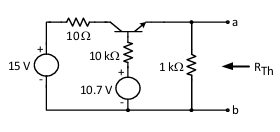
\includegraphics[]{figs/Q.41.png}
    \caption{}
    \label{fig:17}
\end{figure}
\hfill{(GATE EE 2018)}

\item As shown in the figure, C is the arc from the point (3,0) to the point (0,3) on the circle $x^2 + y^2 = 9$. The value of the integral $\int_C (y^2 + 2yx)dx + (2xy + x^2)dy$ is \_\_\_\_\_\_\_\_\_\_ (up to 2 decimal places).
\begin{figure}[H]
    \centering
    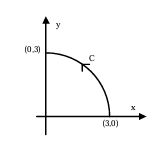
\includegraphics[]{figs/Q.42.png}
    \caption{}
    \label{fig:18}
\end{figure}
\hfill{(GATE EE 2018)}

\item Let $f(x) = 3x^3 - 7x^2 + 5x + 6$. The maximum value of $f(x)$ over the interval $[0, 2]$ is \_\_\_\_\_\_\_\_\_\_ (up to 1 decimal place).

\item Let A = \myvec{
    1 & 0 & -1 \\
    -1 & 2 & 0 \\
    0 & 0 & -2
}
 and $B = A^3 - A^2 - 4A + 5I$, where $I$ is the $3 \times 3$ identity matrix. The determinant of $B$ is \_\_\_\_\_\_\_\_\_\_ (up to 1 decimal place).
 \hfill{(GATE EE 2018)}

\item The capacitance of an air-filled parallel-plate capacitor is 60 pF. When a dielectric slab whose thickness is half the distance between the plates, is placed on one of the plates covering it entirely, the capacitance becomes 86 pF. Neglecting the fringing effects, the relative permittivity of the dielectric is \_\_\_\_\_\_\_\_\_\_ (up to 2 decimal places).
\hfill{(GATE EE 2018)}

\item The unit step response $y(t)$ of a unity feedback system with open loop transfer function $G(s)H(s) = \dfrac{K}{(s+1)^2(s+2)}$ is shown in the figure. The value of $K$ is \_\_\_\_\_\_\_\_\_\_ (up to 2 decimal places).
\begin{figure}[H]
    \centering
    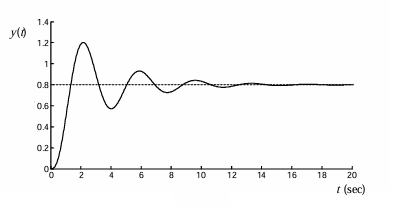
\includegraphics[]{figs/Q.46.png}
    \caption{}
    \label{fig:19}
\end{figure}
\hfill{(GATE EE 2018)}

\item A three-phase load is connected to a three-phase balanced supply as shown in the figure. If $V_{an} = 100\angle0^\circ$ V, $V_{bn} = 100\angle-120^\circ$ V and $V_{cn} = 100\angle-240^\circ$ V (angles are considered positive in the anti-clockwise direction), the value of R for zero current in the neutral wire is \_\_\_\_\_\_\_\_\_\_ $\Omega$ (up to 2 decimal places).
\begin{figure}[H]
    \centering
    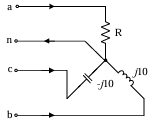
\includegraphics[]{figs/Q.47.png}
    \caption{}
    \label{fig:20}
\end{figure}
\hfill{(GATE EE 2018)}

\item The voltage across the circuit in the figure, and the current through it, are given by the following expressions:
\begin{align*}
v(t) &= 5 - 10 \cos(\omega t + 60^\circ) \, \text{V} \\
i(t) &= 5 + X \cos(\omega t) \, \text{A}
\end{align*}
where $\omega = 100\pi$ radian/s. If the average power delivered to the circuit is zero, then the value of $X$ (in Ampere) is \_\_\_\_\_\_\_\_\_\_ (up to 2 decimal places).
\begin{figure}[H]
    \centering
    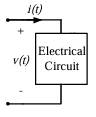
\includegraphics[]{figs/Q.48.png}
    \caption{}
    \label{fig:21}
\end{figure}
\hfill{(GATE EE 2018)}

\item A phase controlled single phase rectifier, supplied by an AC source, feeds power to an R-L-E load as shown in the figure. The rectifier output voltage has an average value given by $V_{in} = \dfrac{V_m}{2\pi} (3 + \cos\alpha)$, where $V_m = 80\pi$ volts and $\alpha$ is the firing angle. If the power delivered to the lossless battery is 1600 W, $\alpha$ in degree is \_\_\_\_\_\_\_\_\_\_ (up to 2 decimal places).
\begin{figure}[H]
    \centering
    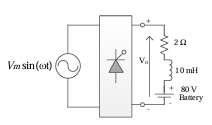
\includegraphics[]{figs/Q.49.png}
    \caption{}
    \label{fig:22}
\end{figure}
\hfill{(GATE EE 2018)}

\item The figure shows two buck converters connected in parallel. The common input dc voltage for the converters has a value of 100 V. The converters have inductors of identical value. The load resistance is 1 $\Omega$. The capacitor voltage has negligible ripple. Both converters operate in the continuous conduction mode. The switching frequency is 1 kHz, and the switch control signals are as shown. The circuit operates in the steady state. Assuming that the converters share the load equally, the average value of $i_{S1}$, the current of switch S1 (in Ampere), is \_\_\_\_\_\_\_\_\_\_ (up to 2 decimal places).
\begin{figure}[H]
    \centering
    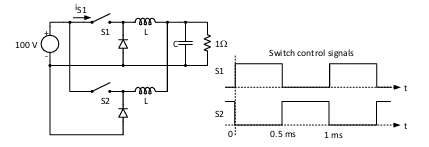
\includegraphics[]{figs/Q.50.png}
    \caption{}
    \label{fig:23}
\end{figure}
\hfill{(GATE EE 2018)}

\item A 3-phase 900 kVA, 3 kV / $\sqrt{3}$ kV ($\Delta$/Y), 50 Hz transformer has primary (high voltage side) resistance per phase of 0.3 $\Omega$ and secondary (low voltage side) resistance per phase of 0.02 $\Omega$. Iron loss of the transformer is 10 kW. The full load \% efficiency of the transformer operated at unity power factor is \_\_\_\_\_\_\_\_\_\_ (up to 2 decimal places).
\hfill{(GATE EE 2018)}

\item A 200 V DC series motor, when operating from rated voltage while driving a certain load, draws 10 A current and runs at 1000 r.p.m. The total series resistance is 1 $\Omega$. The magnetic circuit is assumed to be linear. At the same supply voltage, the load torque is increased by 44\%. The speed of the motor in r.p.m. (rounded to the nearest integer) is \_\_\_\_\_\_\_\_\_\_.
\hfill{(GATE EE 2018)}

\item A dc to dc converter shown in the figure is charging a battery bank, B2 whose voltage is constant at 150 V. B1 is another battery bank whose voltage is constant at 50 V. The value of the inductor, L, is 5 mH and the ideal switch, S is operated with a switching frequency of 5 kHz with a duty ratio of 0.4. Once the circuit has attained steady state and assuming the diode D to be ideal, the power transferred from B1 to B2 (in Watt) is \_\_\_\_\_\_\_\_\_\_ (up to 2 decimal places).
\begin{figure}[H]
    \centering
    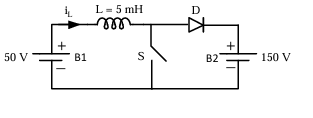
\includegraphics[]{figs/Q.53.png}
    \caption{}
    \label{fig:24}
\end{figure}
\hfill{(GATE EE 2018)}

\item The equivalent circuit of a single phase induction motor is shown in the figure, where the parameters are $R_1=R_2'=X_{l1}=X_{l2}'=12 \, \Omega, X_M=240 \, \Omega$ and s is the slip. At no-load, the motor speed can be approximated to be the synchronous speed. The no-load lagging power factor of the motor is \_\_\_\_\_\_\_\_\_\_ (up to 3 decimal places).
\begin{figure}[H]
    \centering
    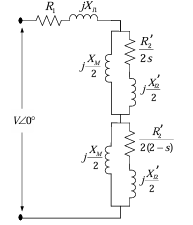
\includegraphics[]{figs/Q.54.png}
    \caption{}
    \label{fig:25}
\end{figure}
\hfill{(GATE EE 2018)}

\item The voltage $v(t)$ across the terminals $a$ and $b$ as shown in the figure, is a sinusoidal voltage having a frequency $\omega = 100$ rad/s. When the inductor current $i(t)$ is in phase with the voltage $v(t)$, the magnitude of the impedance $Z$ (in $\Omega$) seen between the terminals $a$ and $b$ is \_\_\_\_\_\_\_\_\_\_ (up to 2 decimal places).
\begin{figure}[H]
    \centering
    
\includegraphics[]{figs/Q.55.png}
    \caption{}
    \label{fig:26}
\end{figure}
\hfill{(GATE EE 2018)}

\end{enumerate}

\end{document}